\section{Experimentos e Resultados}

Para avaliar o impacto dos hiperparâmetros no desempenho da MLP treinada com gradiente descendente em lote completo sobre o conjunto MNIST, executou-se uma varredura univariada a partir da configuração de referência ($\alpha = 0{,}1$, $200$ épocas, $h = 64$ neurônios e semente $42$), resumida na Tabela~\ref{tab:experimentos}. Observa-se que a taxa de aprendizado exerce o efeito mais acentuado: valores reduzidos ($\alpha \in \{0{,}001; 0{,}01\}$) praticamente impedem a convergência em $200$ épocas, enquanto $\alpha = 0{,}5$ reduz a perda para $0{,}2585$ e eleva a acurácia de teste para $92{,}43\%$ em apenas $280{,}6$~s. O aumento do número de épocas promove ganhos consistentes com crescimento quase linear do tempo de execução, atingindo $90{,}21\%$ em $500$ épocas ($729{,}3$~s). Já a expansão da camada escondida apresenta retornos decrescentes: de $h = 4$ para $h = 256$, a acurácia sobe de $69{,}26\%$ para $87{,}63\%$, mas o custo computacional cresce mais de dez vezes ($922{,}4$~s).

\begin{table}[t]
\centering
\small
\setlength{\tabcolsep}{4pt}
\begin{tabular}{lrrrr}
\toprule
Grupo & Valor & Perda & Acurácia (\%) & Tempo (s) \\
\midrule
Taxa ($\alpha$) & 0,001 & 2,3016 & 12,71 & 353,5 \\
                & 0,01 & 2,2840 & 30,61 & 355,7 \\
                & 0,1$^\dagger$ & 0,5320 & 86,11 & 355,5 \\
                & \textbf{0,5} & \textbf{0,2585} & \textbf{92,43} & \textbf{280,6} \\
\midrule
Épocas          & 50 & 2,1144 & 44,28 & 113,9 \\
                & 100 & 1,0912 & 76,28 & 196,4 \\
                & 200$^\dagger$ & 0,5320 & 86,11 & 355,5 \\
                & \textbf{500} & \textbf{0,3417} & \textbf{90,21} & \textbf{729,3} \\
\midrule
Escondida ($h$) & 4 & 0,9421 & 69,26 & 84,7 \\
                & 16 & 0,6374 & 83,74 & 115,9 \\
                & 64$^\dagger$ & 0,5320 & 86,11 & 355,5 \\
                & \textbf{256} & \textbf{0,4755} & \textbf{87,63} & \textbf{922,4} \\
\bottomrule
\end{tabular}
\caption{Resultados da varredura de hiperparâmetros no conjunto de teste MNIST. O símbolo $^\dagger$ marca a configuração de referência ($\alpha = 0{,}1$, $200$ épocas, $h = 64$, semente $42$), e o negrito destaca o melhor resultado de cada bloco.}
\label{tab:experimentos}
\end{table}

Duas configurações da varredura superaram a meta de $90\%$ de acurácia no teste: $500$ épocas ($90{,}21\%$ em $729{,}3$~s) e $\alpha = 0{,}5$ ($92{,}43\%$ em $280{,}6$~s), sendo esta última superior tanto em precisão quanto em eficiência. A Figura~\ref{fig:curvas} ilustra a evolução da perda de entropia cruzada e da acurácia ao longo das $200$ épocas para os quatro valores de $\alpha$. Com $\alpha = 0{,}5$, a perda cai abruptamente nas iterações iniciais e a acurácia cresce de forma acelerada até atingir $92{,}43\%$. A referência ($\alpha = 0{,}1$) apresenta queda moderada e contínua, ao passo que $\alpha = 0{,}01$ progride lentamente e $\alpha = 0{,}001$ permanece quase estagnado próximo à perda inicial de um classificador uniforme ($\ln 10 \approx 2{,}3026$).

% [TODO: se houver melhor modelo dedicado >=90% finalizado, atualizar figura e métricas]
\begin{figure}[t]
\centering
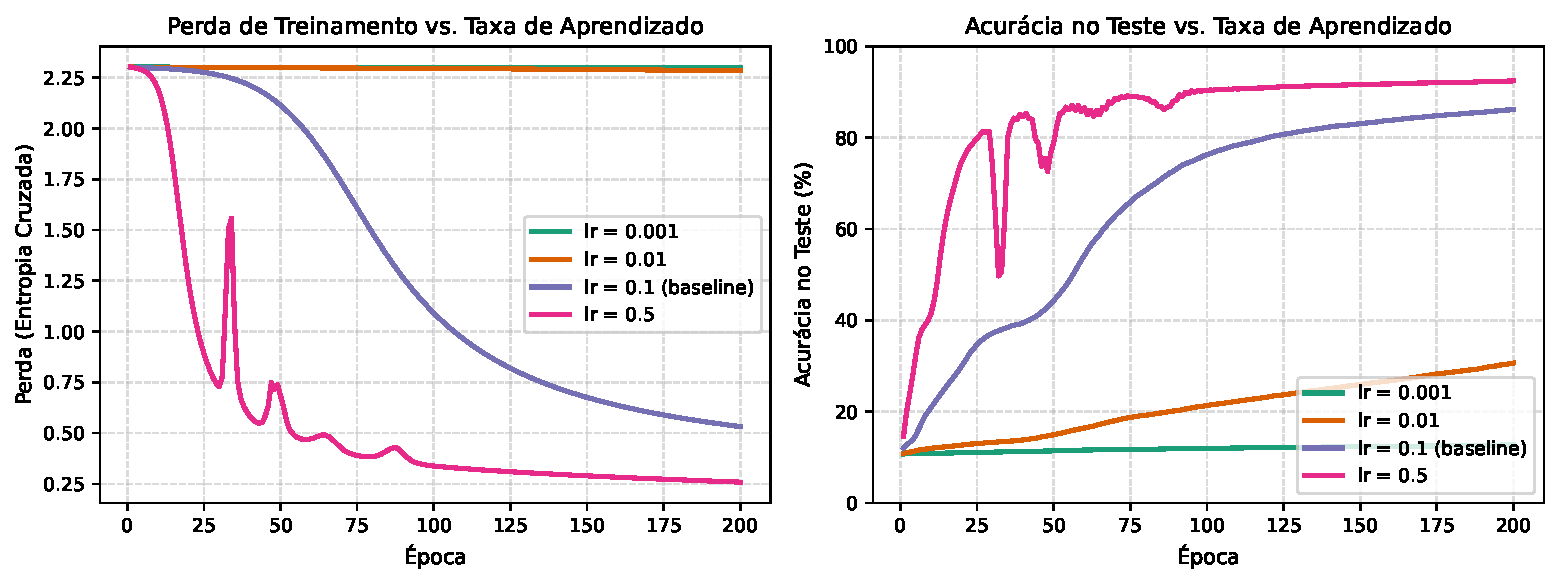
\includegraphics[width=\columnwidth]{figures/sweep_learning_rate.pdf}
\caption{Curvas de perda e acurácia ao longo de $200$ épocas para $\alpha \in \{0{,}001; 0{,}01; 0{,}1; 0{,}5\}$ com $h = 64$, destacando a convergência da melhor configuração ($\alpha = 0{,}5$, $92{,}43\%$).}
\label{fig:curvas}
\end{figure}

\subsection{Análise Qualitativa na Interface Interativa}

Para complementar a avaliação quantitativa, carregaram-se os pesos do melhor modelo ($\ge 90\%$ de acurácia) na interface web de \texttt{server.py} (\texttt{http://localhost:5001}), desenhando-se dígitos manuscritos na grade $28 \times 28$. Nos testes interativos, [TODO: preencher com os 3+ dígitos desenhados na interface, indicando a classe predita e a confiança Softmax obtida em cada caso]. Quanto aos padrões de acerto e erro, [TODO: preencher com os 3+ dígitos desenhados na interface --- quais dígitos foram reconhecidos com maior confiabilidade e quais pares sofreram confusão]. Esse comportamento reflete propriedades estruturais da MLP: como cada pixel de entrada possui pesos independentes, a predição depende fortemente da espessura do traço e da centralização na grade $28 \times 28$, evidenciando a sensibilidade da rede totalmente conectada a pequenas translações em relação ao padrão do MNIST.
